\documentclass[12pt]{article}
\usepackage[final]{graphicx}

\usepackage{float}
%\usepackage[caption = false]{subfig}

\usepackage[lofdepth,lotdepth]{subfig}

\title{Lane Detecion Project}
\author{Mingrui Wu}
\date{}

\begin{document}

\maketitle


\section{Camera Calibration}
The colde for this step is in py/camera\_calibration.py. Camera clibaration is done by following the materials taught in the class. Twenty chess board images are provided in the camera\_cal folder. 
\begin{enumerate}
	\item For each image, find the inner corners by $cv2.findChessboardCorners$. For this function the number of corners in x and y direstions are 9 and 6 respectively.
	\item Append the corners found in the previous step to an array $imgpoints$, at the same time append pre-calculated mesh grid points to another array $objp$
	\item Having scanned all the twenty images, apply $cv2.calibrateCamera$ to calcuate the calibration paramters
	\item For each of the twenty images, apply $cv2.undistort$ to correction the distortion, where the calibration parameters needed by this function are computed in the last step.
\end{enumerate}
	 
An example of camera calibration is given in image \ref{camera_calib}. The two images in the left column are the inpute images, while the two in the right column are the images after distortion correction.

\begin{figure}[h]
\centering
\subfloat[input image]{
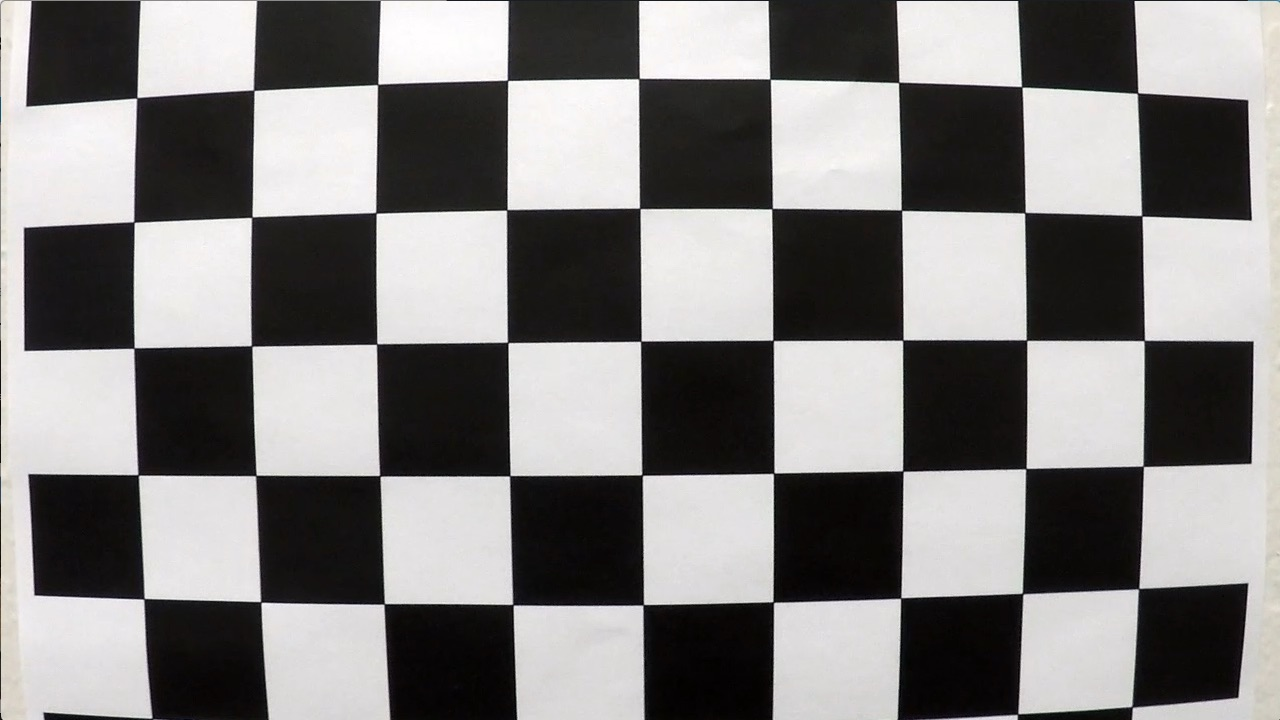
\includegraphics[width=0.4\textwidth]{calibration1.jpg}
\label{fig:input}}
\qquad
\subfloat[undistorted image]{
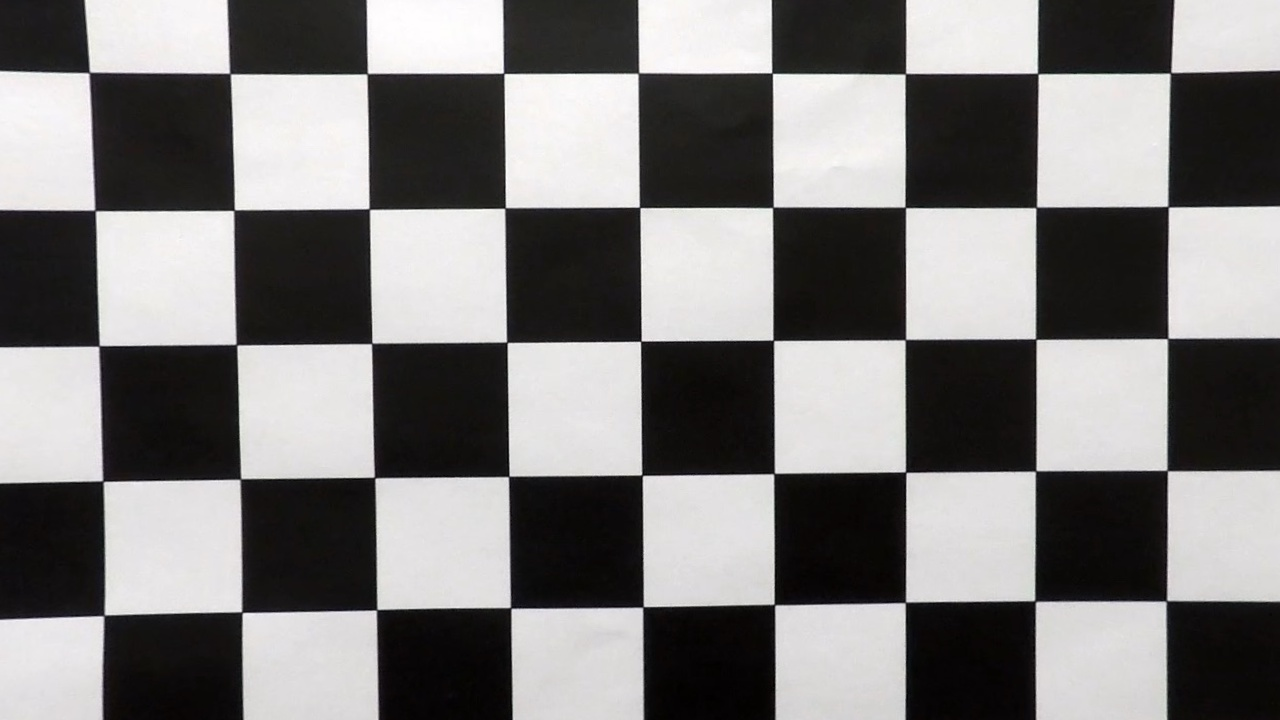
\includegraphics[width=0.4\textwidth]{undist_calibration1.jpg}
\label{fig:camera_calib}}
\qquad
\subfloat[input image]{
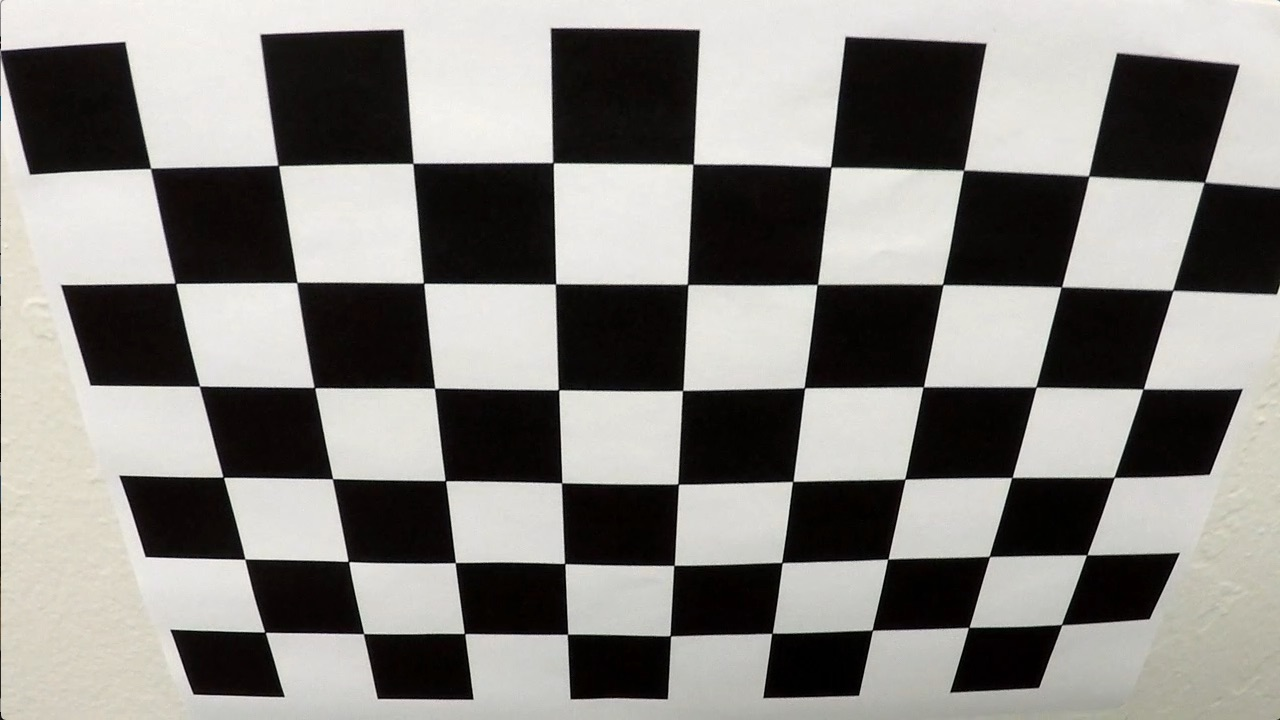
\includegraphics[width=0.4\textwidth]{calibration2.jpg}
\label{fig:input}}
\qquad
\subfloat[undistored image]{
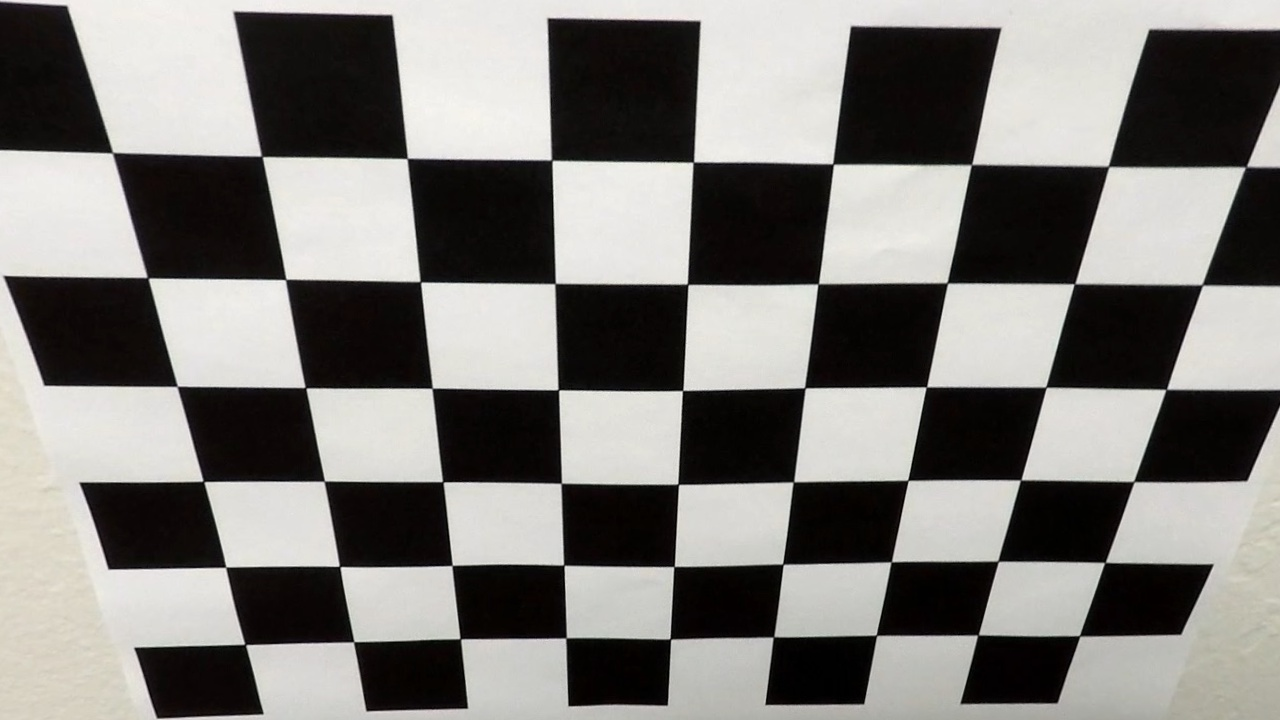
\includegraphics[width=0.4\textwidth]{undist_calibration2.jpg}
\label{fig:camera_calib}}
\caption{Camera calibration}
\end{figure}

The undisorted images for all the twenty images provided in the  camera\_cal folder can be found in  camera\_cal/calib\_result folder.
  
    
\section{Pipline}
In my code, LaneDetector is the class for performing lane detection. The code is in py/lane\_detector.py. Within this class, the member function LaneDetector.lane\_detect describes the whole pipeline.

Take the input image Fig \ref{fig:input} as an example, the whole piple line consists of the following steps:

\begin{enumerate}
	\item \textbf{Loading pre-computed parameters.} First, an object of the LandDetectParam class is created. And this object contains all the parameters needed for the whole lane detection pipeline. In particular, it will load the pre-calculated paramters for camera calibration and perspective transform. The code for this part is in py/lane\_detect\_param.py
	 
	\item \textbf{Distortion correction.} Using the pre-calculated camera calibration parameters mentioned in the last section, the first step is to apply $cv2.undistort$ to the input image to get the undistorted image. The undistorted result for \ref{fig:input} is given in \ref{fig:undistort}

	\item  \textbf{Binary thresholding}  BinaryThresholder is the class for this step. The code is in py/binar\_thresholding.py. Following the class, this done by combining the result from gradient and color transformation.
		\begin{enumerate}
			\item \textbf{Sobel gradient} The input image is first transformed to a gray scale image. And then the Sobel operator is applied to the grayscale image to obtain the gradient image. Then based on the gradient strengh in x and y directions, the magnitude and the direction of the gradient at each pixel, binary thresholding is performed.

			\item  \textbf{S space} The input image is transformed into HLS space first. Then binary thresholding is performed based on the S-space value.
			\item \textbf{Combination} The two binary images are combined by OR operation. In addition, the pixels whose S-space value is lower than a threshold are filtered out.
			
			\item \textbf{RGB filtering} If the image obtained in the last step still have many pixeld obtained (more than 40\%), then the pixels whose RGB value is lower than a threshold are filtered out.
		\end{enumerate}
	The binarization example is given in \ref{fig:binarization}
	
	\item \textbf{Perspective transform.} 
		\begin{enumerate}
			\item \textbf{Pre-calculation.} Parameters for perspective transform are pre-calcuated. The code is in py/camera\_calibration.py. For source points and destinations points are selected manually. Then the matrices for both perspective and inverse perspective transform are obtained by applying the function $cv2.getPerspectiveTransform$. This is done by applying $cv2.warpPerspective$ function.
			
			\item \textbf{Perspective transform.} The function $cv2.warpPerspective$ is applied to the binary image obtained in the binary thresholding step.
		\end{enumerate}
	The wapred image is given in \ref{fig:warped}.
	
	\item \textbf{Polynomial fit.} Having obtained the warped image in the last step, PolyFitter is the class for identifying lane pixels and curve fitting. The code is in py/ply\_fitter.py. There are two sub steps:
		\begin{enumerate}
			\item {Lane pixel identifcation} When processing an individual image or the first frame of a video, the approach based on histogram provided in the class material is applied. First the left and right starting points are selected based on the maximum column sum of the left half and right half of the binary image. Then for left and right lane, we search along the y direction for the non-zero pixels around the current columns. And the staring points are updated based on the mean position of the non-zero pixels that have been found. This is coded in the function PolyFitter.find\_lane\_pixels. When processing videos, the lane pixels are searched along the polynomial curves obtained from the previous frame. The code for this in the function PolyFitter.search\_around\_poly.
			
			\item \textbf {Poly fit.} Having obtained the lane pixels, numpy.polyfit is applied to fit a quadratic curve.
		\end{enumerate}
	The fitted polynomial curves are given in the image \ref{fig:polyfit}.
	
	
	\item \textbf{Calculate radius of curvature and the position of the vehicle.} 
		\begin{enumerate}
			\item \textbf{Computing the radius of curature.} The radius of curvature of left and right lanes can be calculated once we have the parmaters of the fitted polynomial curves. But here the curves are fitted by the salced the coordinates of the lane pixels. The funtion is PolyFitter.meansure\_curvature\_real. Then the mean of these two radius of curvature is returned as the raidus of curvature of the road. 
			
			\item textbuf{Computing the position of the vehicle.} Based on the two fitted polynomail curves, we can get the x coordinates of the two points corresponding to the maximum y value of the image. Then the mean value of these two x coordinates is the estimation of the vehicle's position. Note that here we need to scale the result to reflect the real distance rather than the number of pixels. The code is given in LaneDetector.compute\_vehicle\_pos.
		\end{enumerate}
	
	\item \textbf{Render lane image}. Having obtained all the information in the previous steps, I render the lane image by filling the regions surronded by the lane points. An example of the lane image is given in \ref{fig:lane}.
			
\end{enumerate}

\begin{figure}[h]
\centering
\subfloat[input image]{
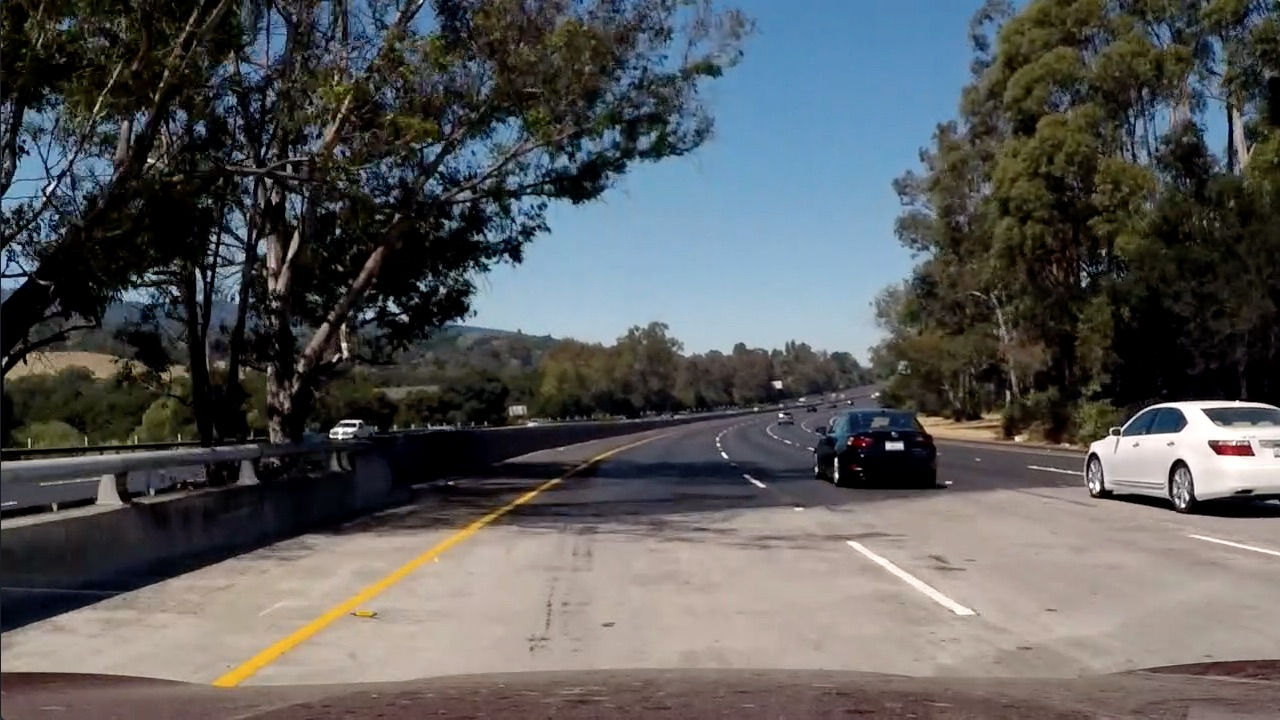
\includegraphics[width=0.4\textwidth]{test5.jpg}
\label{fig:input}}
\qquad
\subfloat[undistorted image]{
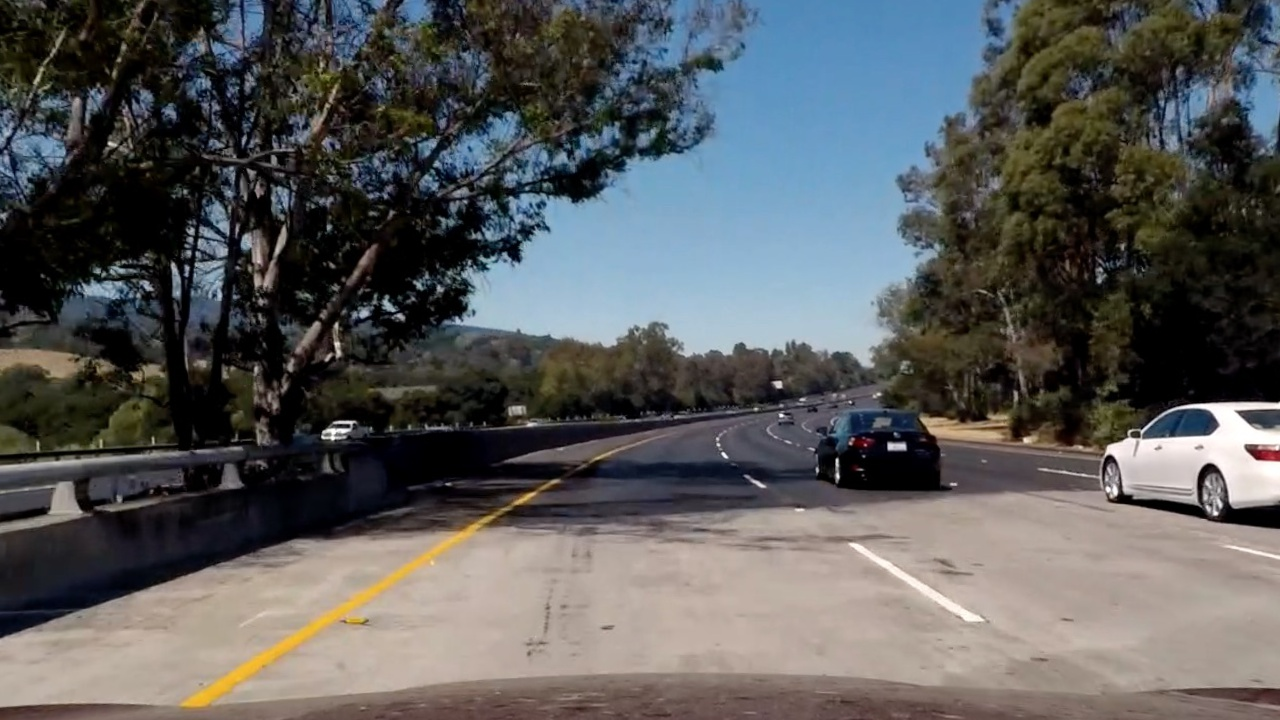
\includegraphics[width=0.4\textwidth]{undist_test5.jpg}
\label{fig:undistort}}
\qquad
\subfloat[binary image]{
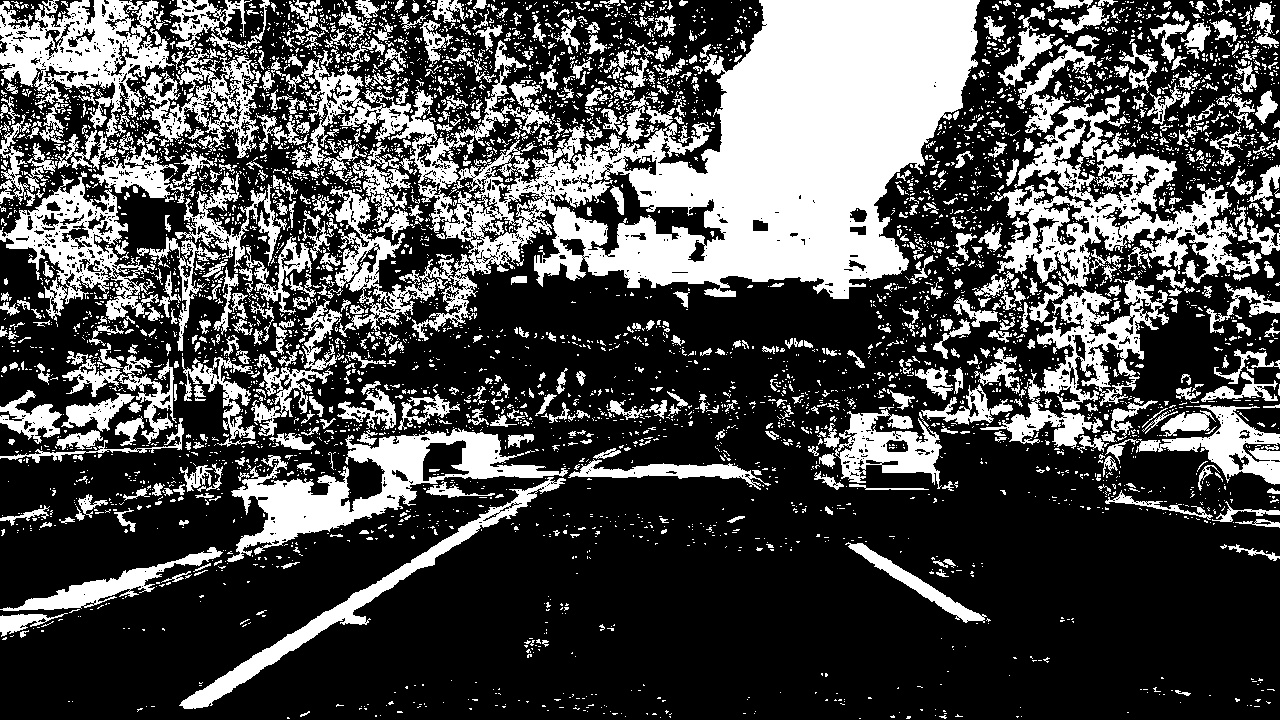
\includegraphics[width=0.4\textwidth]{bin_test5.jpg}
\label{fig:binarization}}
\qquad
\subfloat[warped image]{
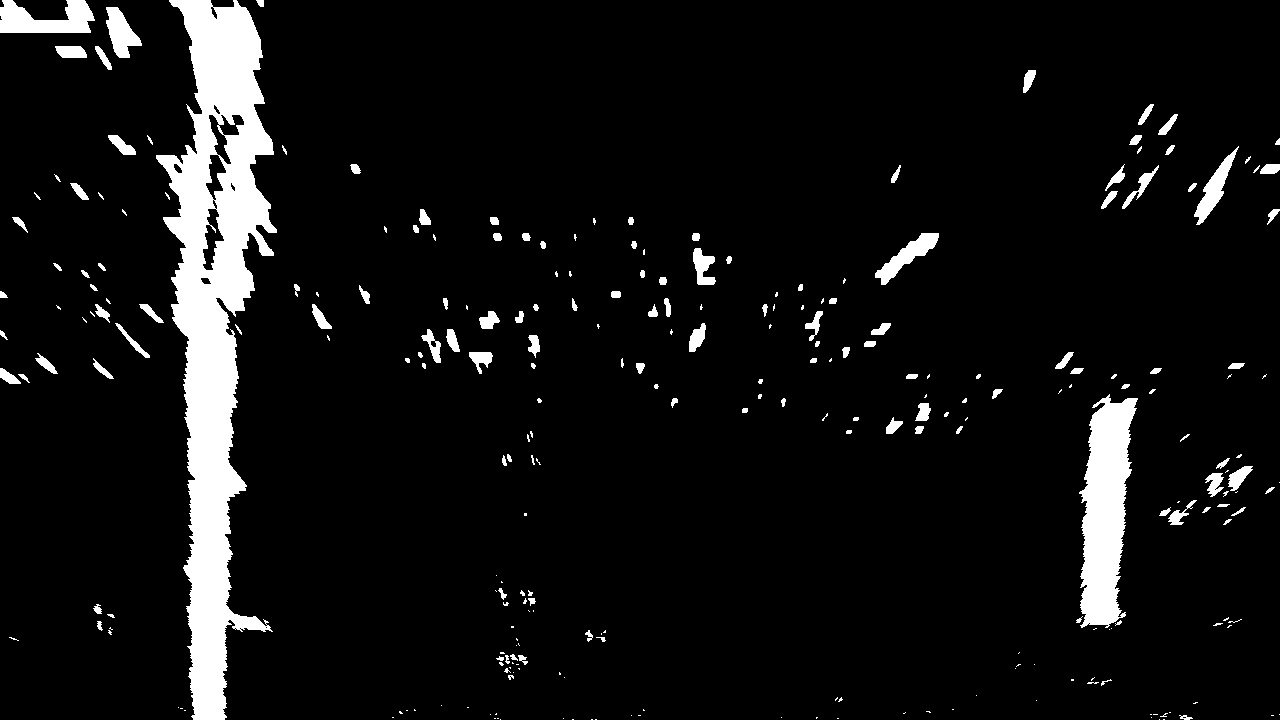
\includegraphics[width=0.4\textwidth]{warp_test5.jpg}
\label{fig:warped}}
\qquad
\subfloat[poly image]{
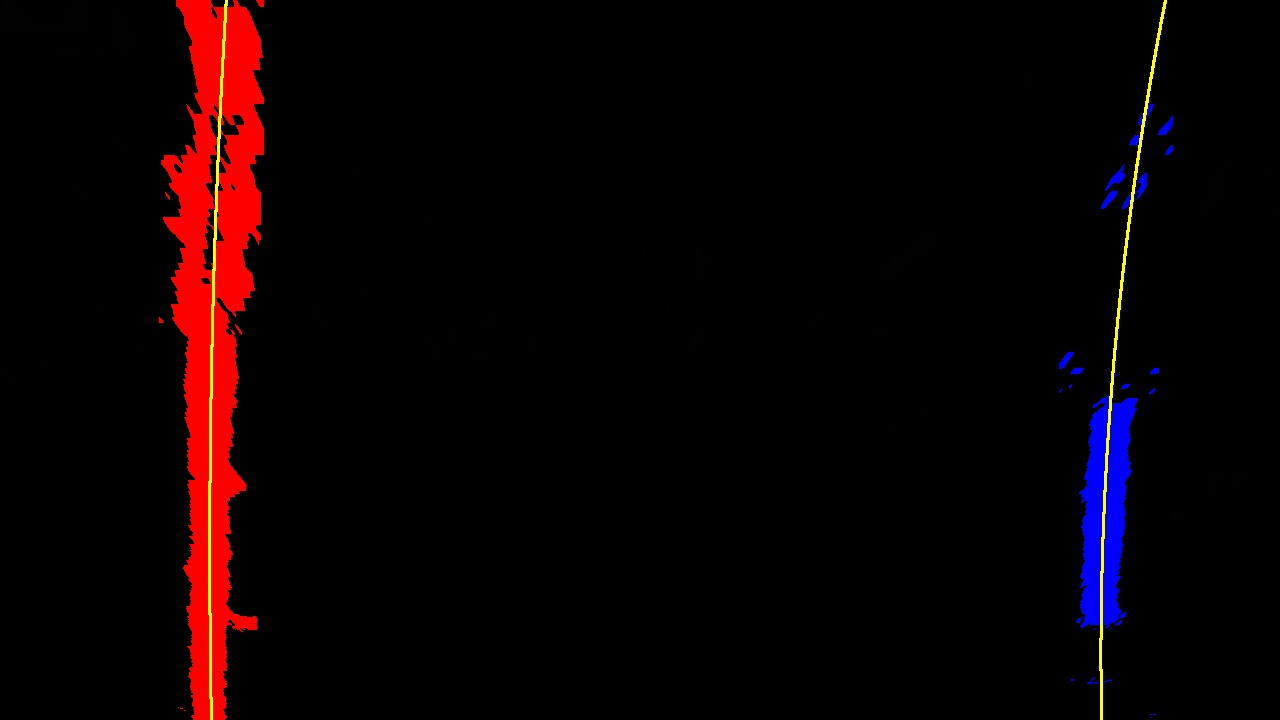
\includegraphics[width=0.4\textwidth]{fit_test5.jpg}
\label{fig:polyfit}}
\qquad
\subfloat[lane image]{
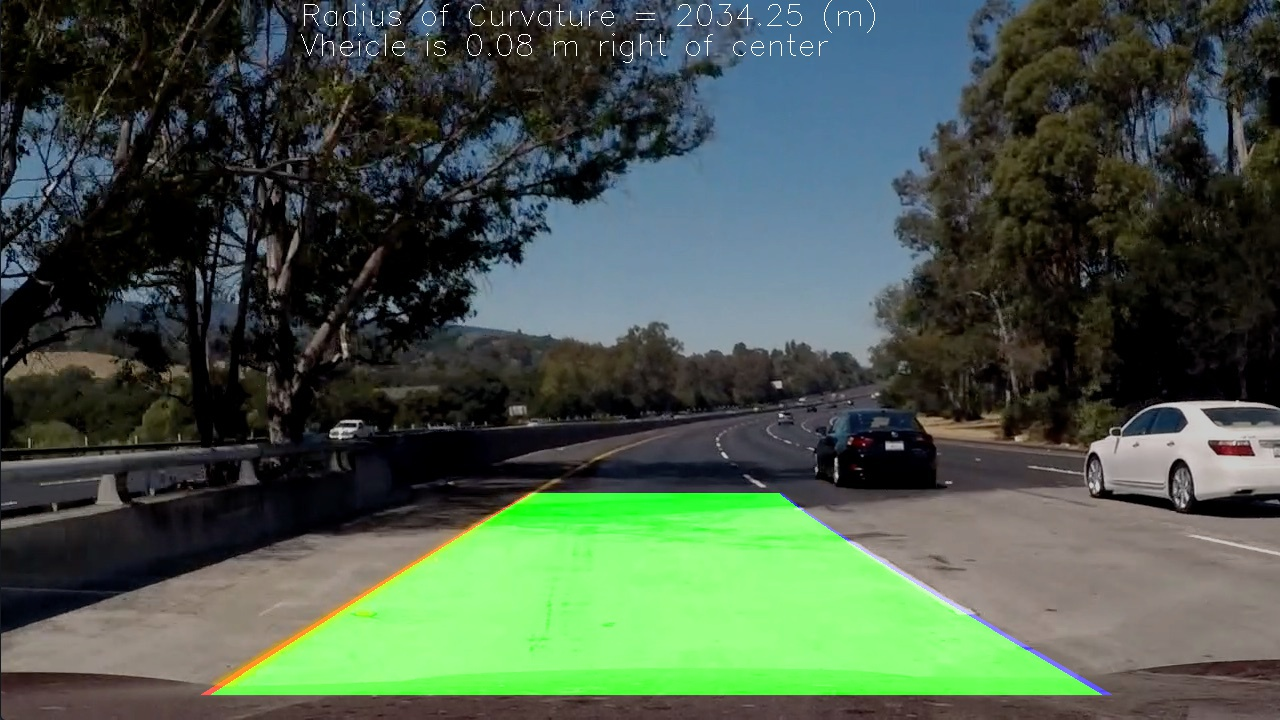
\includegraphics[width=0.4\textwidth]{lane_test5.jpg}
\label{fig:lane}}
\caption{Lane detection pipeline}
\end{figure}

\section{Full extent of lane lines}
This section explains the last step of the pipeline. This in turn contains two steps. 

\subsection{Grouping line segments into left and right}
In the second last step, a set of line segments are obtained by Hough transform. These line segments are grouped into left and right lines respectively, based on the slopes. The line segments with negative slopes are put into the left group, while the line segments with the positive slopes are put into the right group. In implementation, to filter out some noisy line segments, only the line segments whose slopes are within the given slope ranges are considered, while the other line segments are ignored. The slope ranges are parameters need to be tuned. And there is one slope range for the left group and the right group respectively.

\subsection{Forming the full lane lines}
Having obtained left and right groups of line segments, we need to form one line from each group. Two approaches have been tried.

\subsubsection{Avearing the line segments in one group}
For each group of line segments, this approach simply builds the full extent line by averaging the slopes and interceptions of the line segments in the group. This approach works in most cases. However it is not robust since it can be eaily disturbed by some nosisy slope or interception values. For example, if some line segments' slopse or/and interceptions are far away from the ground true, even those short segments are located within the true lane lines, averaging can still result in the slopes/interceptions that are quite different from those of the true land lines. This problem can be alleviated by fine tuning the parameters, but I am trying to find some better approaches.

\subsubsection{Robust line fitting with RANSAC}
The above approach is not robust since averaging slopes and interceptions can be easily disturbed by outlier segments even when those outliers are located within the true lane lines.

Based on the above observation, instead of computing the slopes and interceptions by averaing, I turn to fit one line robustly for each group, left and right respectively. So for each group, we just need to fine one line that are close to the end points of the line segments in the group. This can overcome the problem in the averaging approach: as long as the line segments are within the true lane lines, this can produce the ideal result even when the slopes/interceptions of those segments are quite different from those of the true lane lines. For the nosity line segments that are located far away from the lane lines, RANSAC algorithm can ignore them automatically.

This approach works very well on the test videos. It gives good estimation in almost all the frames.



\section{Problems and possible improvements}
The above pipeline works pretty well on the given test images and test videos. However, it breaks on some parts of the challenging video, challenge.mp4. The reason is that in the chanllenge.mp4, there are some strong edges: the car itself and the color change of the road. A failure example is shown in Fig \ref{fig:failure}. 

I tried to fine tunning the parameters for color detection, since the pixles around those edges are neither white nor yellow. However, mannully tunning the parameters can be suffering. It may improve the results on some particular frames while break the results on some other frames. Probably a more principaled way like building a trained model which considers both color and edge information can get a better result.


\end{document}
